\section{Results}
\subsection{Main Result}
We show that, given large N, for an SBM the relative efficiency between $\hat{P}$ and $\bar{A}$ is:
\begin{equation}
RE_{ij} =\frac{Var(\hat{P}_{ij})}{Var(\bar{A}_{ij})} = \frac{1/\rho_i + 1/\rho_j}{N}
\end{equation}
This comes from a proof (outlined in section 4.X) for the variance of $\hat{P}_{ij}$ under the condition that N is large:
\begin{equation}
Var(\hat{P}_{ij}) = \frac{(1/\rho_i + 1/\rho_j)P_{ij}(1-P_{ij})}{NM}
\end{equation}
Further, knowing that $\bar{A}_{ij}$ is the estimator of the Bernoulli parameter $P_{ij}$ from M samples, with variance $P_{ij}(1-P_{ij})/M$, this yields the above result.

This result implicates then that for large graphs that follow a stochastic block model, a better estimate for the mean graph, under mean squared error (MSE), is the $\hat{P}$ estimate.
\subsection{Validation with Simulations}
To demonstrate the above result for the variance of $\hat{P}$ and relative efficiency (Equations x.x and x.x), we simulate random graphs from an SBM with parameters:
\begin{equation*}
B = \begin{bmatrix}
.42 & .2 \\
.2 & .7 
\end{bmatrix}
,\qquad \rho = \begin{bmatrix}
.5 & .5
\end{bmatrix}
\end{equation*}

From this model we perform simulated studies by sampling $M$ adjacency matrices with $N$ vertices to calculate both $\bar{A}$ and $\hat{P}$.  With these estimators for $P$, we can calculate the MSE of each block region in the model, defined as the elements of the adjacency matrix that have the same edge-wise probability.  This simulation is then repeated 1000 times and the estimates for variance and relative efficiency are averaged over the trials.  We then confirm that these simulation errors match with our predictions.

Using this model, we first aim to verify equation XX for $Var(\hat{P}_{ij})$.  Figure 1a demonstrates that as N increases, the $Var(\hat{P}_{ij})$ for this block model converges to our estimate, represented as the dotted lines.  Further Figure 1b illustrates that the result holds independently of the value of M, and that high M is not a necessary condition for our estimate.
\begin{figure}[!htb]
	\centering
	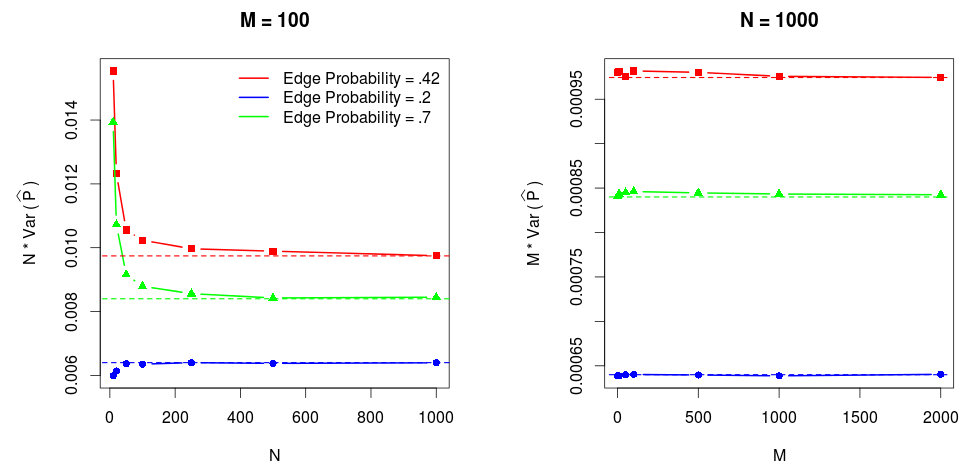
\includegraphics[width=16cm]{VarNM_rho.PNG}
	\caption{Simulation results. (a) N*Var$(\hat{P})$ and  (b) M*Var$(\hat{P})$  calculated from edges with associated edge probabilities, while increasing N and M, respectively.  Observe that the simulated values asymptotically, in N, converge to the predictions, represented by the dotted lines.}
	\label{fig:plot1}
\end{figure}

To verify the result for relative efficiency, we again use the previous model for simulations to compare the estimators $\bar{A}$ and $\hat{P}$.  As Figure 2 demonstrates, for large N equation X holds true. 
\begin{figure}[!htb]
	\centering
	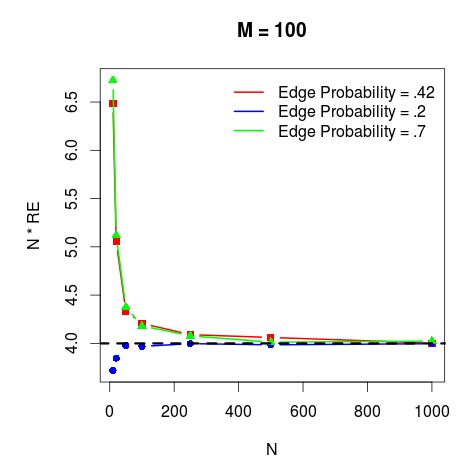
\includegraphics[width=9cm]{RE.PNG}
	\caption{N*RE calculated from edges with associated edge probabilities.  Observe that the simulated values asymptotically converge to the predictions, represented by the dotted line.}
	\label{fig:plot1}
\end{figure}

To confirm that equations x and x hold with respect to $\rho$ values, we now examine simulations where the $\rho$ vector for the SBM  is varied, while fixing N and M.

\begin{equation*}
B = \begin{bmatrix}
.42 & .2 \\
.2 & .7 
\end{bmatrix}
,\qquad \rho = \begin{bmatrix}
\rho_1 & \rho_2
\end{bmatrix}
,\qquad N = 500,\qquad M = 100
\end{equation*}

Figure 3 demonstrates the effect of different block membership, $\rho$, values on both Var$(\hat{P})$ and RE.  These simulated results again match well for the predictions from equation x and x, with a mean deviation of 3.7e-7, and 1.6e-4, respectively.
\begin{figure}[!htb]
	\centering
	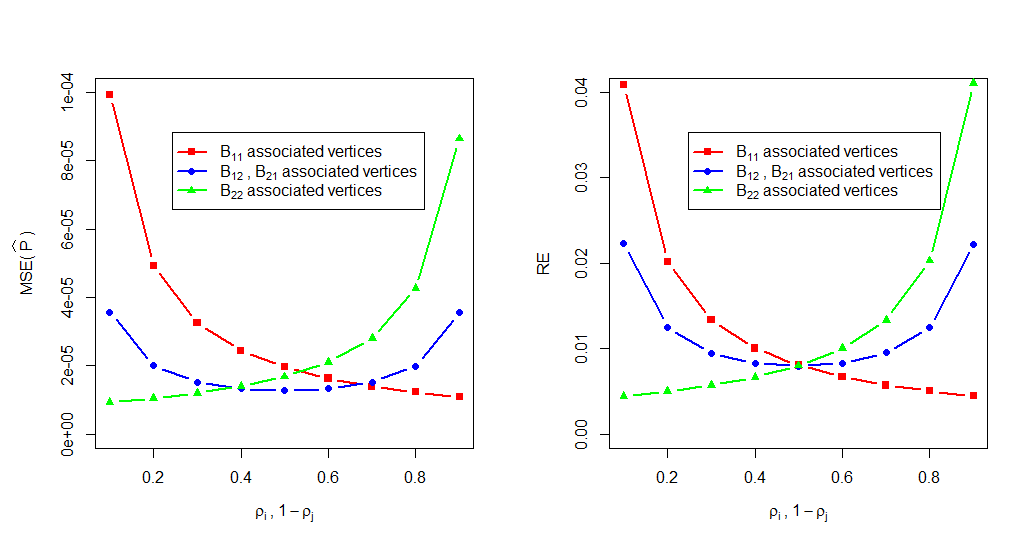
\includegraphics[width=16cm]{VarRE.PNG}
	\caption{Simulated results for (a) Var$(\hat{P})$ and (b) RE calculated from edges with associated edge probabilities. The simulated values for the variance and RE measurements deviated from the predictions with a mean of 3.7e-7, and 1.6e-4, respectively.}
	\label{fig:plot1}
\end{figure}
\subsection{CoRR Brain Graphs: Cross-Validation}
	
	To demonstate that the $\hat{P}$ estimate is valid under data that does not perfectly follow an SBM, we examine a set of 464 brain connectomes generated from fMRI scans available at the Consortium for Reliability and Reproducibility (CoRR).  Details on this dataset and connectiome generation can be seen in section x.x.  The connectomes generated each have 788 vertices, with anatomical correspondence. To compare $\bar{A}$ and $\hat{P}$ we perform a cross-validation study to examine the impact of the number of available graphs, M.  For each sample size M, we randomly sample M adjacency matrices from the CoRR data set and estimate the mean with both $\bar{A}$ and $\hat{P}$.  We then calculated the MSE of these estimators compared to the test mean, defined to be the $\bar{A}$ estimate of the $464-m$ remaining samples. 
	
	\begin{figure}[!htb]
		\centering
		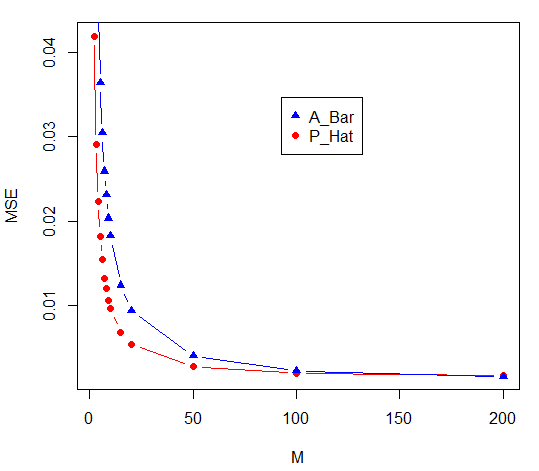
\includegraphics[width=8cm]{XV_MSE.PNG}
		\label{fig:plot1}
		\caption{Mean squared error, calculated through cross-validation, in estimating the mean graph on the CoRR brain graphs.}
	\end{figure} 
\newpage